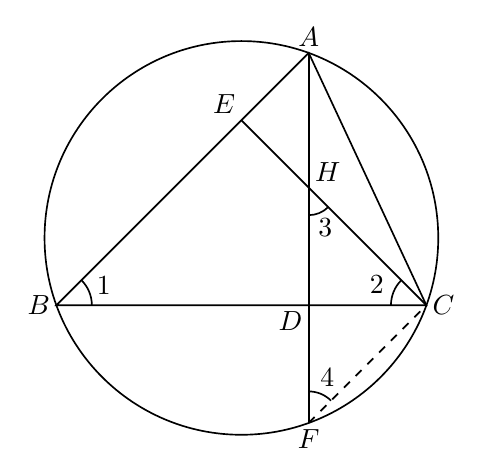
\begin{tikzpicture}[x=1cm,y=1cm,line width=.6pt,font=\normalsize]
\coordinate (O) at (0,0);
\coordinate (A) at (0.8550504,2.3492319);
\coordinate (B) at (-2.3492319,-0.8550504);
\coordinate (C) at (2.3492319,-0.8550504);
\coordinate (D) at (0.8550504,-0.8550504);
\coordinate (E) at (0,1.4941815);
\coordinate (H) at (0.8550504,0.6391311);
\coordinate (F) at (0.8550504,-2.3492319);
\draw (O) circle[radius=2.5cm];
\draw (A)--(B)--(C)--cycle;
\draw (A)--(F);
\draw (C)--(E);
\draw[dashed] (F)--(C);
\draw (B) ++(0:0.45cm) arc[start angle=0,end angle=45,radius=0.45cm];
\draw (C) ++(135:0.45cm) arc[start angle=135,end angle=180,radius=0.45cm];
\draw (H) ++(270:0.35cm) arc[start angle=270,end angle=315,radius=0.35cm];
\draw (F) ++(45:0.4cm) arc[start angle=45,end angle=90,radius=0.4cm];
\node at (-1.749,-0.606) {$1$};
\node at (1.721,-0.595) {$2$};
\node at (1.065,0.131) {$3$};
\node at (1.092,-1.776) {$4$};
\node[above=2pt,inner sep=0pt] at (A) {$A$};
\node[left=2pt,inner sep=0pt] at (B) {$B$};
\node[right=2pt,inner sep=0pt] at (C) {$C$};
\node[below left=2pt,inner sep=0pt] at (D) {$D$};
\node[above left=2pt,inner sep=0pt] at (E) {$E$};
\node[above right=2pt,inner sep=0pt] at (H) {$H$};
\node[below=2pt,inner sep=0pt] at (F) {$F$};
\end{tikzpicture}
